\section{Methodology}\label{sec:methodology}

\subsection{Overview}
This section describes how the experiment was built and run. The design follows one rule: the
two simulated environments may differ only in where their geometry comes from. Everything else,
including the robot model, physics settings, task, reward, randomisation, learning algorithm and
route set, is shared. The photogrammetry world is the method under test; the standard world,
built by hand from tape measurements, is the baseline it is compared against.
Fig.~\ref{fig:pipeline} shows the full pipeline, which has five stages:
\begin{enumerate}
\item Capturing the real room with photogrammetry and checking the model against tape measurements.
\item Building two simulated versions of the room: the photogrammetric mesh, and a standard model
made of simple shapes built from the same tape measurements.
\item Integrating Pepper into the simulator and calibrating it against the real robot.
\item Training navigation policies with SAC under domain randomisation in each world.
\item Deploying one policy from each world on the physical Pepper and comparing the results.
\end{enumerate}

\begin{figure}[t]
\centering
\begin{tikzpicture}[
  node distance=3.5mm and 3mm,
  box/.style={draw, rounded corners=2pt, align=center, font=\scriptsize,
              minimum height=6.5mm, inner sep=2pt},
  photo/.style={box, fill=violet!12},
  std/.style={box, fill=brown!15},
  shared/.style={box, fill=gray!12, text width=0.86\columnwidth},
  real/.style={box, fill=blue!10, text width=0.86\columnwidth},
  arr/.style={-{Stealth[length=2mm]}, thick}]
\node[box, fill=teal!12] (room) {Real room};
\node[photo, below=5mm of room, xshift=-0.27\columnwidth, text width=0.36\columnwidth] (scan)
  {Polycam scan\\ $\rightarrow$ textured mesh};
\node[std, below=5mm of room, xshift=0.27\columnwidth, text width=0.36\columnwidth] (tape)
  {Tape measurements\\ $\rightarrow$ primitive shapes};
\node[photo, below=of scan, text width=0.36\columnwidth] (pw) {Photogrammetry world};
\node[std, below=of tape, text width=0.36\columnwidth] (sw) {Standard world};
\node[shared, below=5mm of $(pw.south)!0.5!(sw.south)$] (train)
  {Identical Pepper model, task, reward, randomisation and SAC configuration (3 seeds per world)};
\node[real, below=of train] (deploy)
  {Pre-registered policy choice $\rightarrow$ zero-shot deployment on the physical Pepper (20 routes)};
\node[shared, below=of deploy] (eval) {Compare SR, SPL, CR and the sim-to-real gap $\Delta$};
\draw[arr] (room) -- (scan.north);
\draw[arr] (room) -- (tape.north);
\draw[arr, dashed] (tape.west) -- node[above, font=\tiny, align=center] {ground truth\\for check} (scan.east);
\draw[arr] (scan) -- (pw);
\draw[arr] (tape) -- (sw);
\draw[arr] (pw.south) -- (pw.south |- train.north);
\draw[arr] (sw.south) -- (sw.south |- train.north);
\draw[arr] (train) -- (deploy);
\draw[arr] (deploy) -- (eval);
\end{tikzpicture}
\caption{The experimental pipeline. The two branches (purple: photogrammetry (method), brown:
standard (baseline)) differ only in the source of the room geometry; every later stage is shared.}
\label{fig:pipeline}
\end{figure}

\subsection{The Photogrammetry Branch}
The target room is a $5.5 \times 4.2$\,m storage room containing a couch, two chairs, a shelf, three
large boxes, a bag, a green pole and a red pole that serves as the navigation goal
(Fig.~\ref{fig:layout}). It was captured with the Polycam application in photo mode on an iPad Pro
11-inch (2nd generation). Over a 10--30 minute session, overlapping photographs were taken while
walking around the room, at several heights, and around each piece of furniture so that it was
seen from all sides. The room lights were on, nothing was moved during the capture, and no
people were in the room. Polycam then processed the photographs into a textured 3D mesh using
photogrammetry (Section~\ref{sec:background}), which was exported as a GLB file. The mesh was
already at metric scale, so no scale correction was applied; the accuracy gate below confirms
this.

A custom import script (\texttt{mesh\_import.py}) converted the mesh into a simulator model in
a repeatable way. It aligned the room with the simulator axes, placed the origin at
the floor corner, smoothed scanning noise with a light Taubin filter, and reduced the mesh to
50{,}000 faces (using Blender) so the physics engine could run it in real time. Every transform was saved to a
manifest file so the import can be reproduced exactly.

Before training, the model had to pass an accuracy gate. Ten room dimensions ($K=10$) were measured
with a tape measure, including room length, width and height, and the heights of the furniture, and
the same dimensions were measured on the mesh. The mean absolute percentage error was
\begin{equation}
\bar{e} = \frac{1}{K}\sum_{k=1}^{K}\frac{|m_k-\hat{m}_k|}{m_k}\times 100\%,
\label{eq:gate}
\end{equation}
where $m_k$ is the tape measurement and $\hat{m}_k$ the mesh measurement. The threshold was the
4.97\% reported for consumer-grade photogrammetry by Alhamadah et al.\
\cite{alhamadah2024photogrammetry}. The reconstruction achieved $\bar{e}=2.12\%$. The largest
errors were on soft objects (couch height 6.85\%, bag height 5.70\%), and the room dimensions
were within about 1\%.

Two problems appeared once Pepper drove on the scanned floor. First, the floor was tilted by
$1.78^\circ$, so the mesh was levelled to $0.01^\circ$. Second, small bumps in the scanned floor
caught Pepper's wheels and left the robot stuck. To fix this, only the \emph{collision} mesh was
flattened below 0.12\,m (high enough to remove the bumps in the scanned floor, but lower than
any real object in the room). The visual mesh, which the depth camera sees, was not changed, and the
accuracy gate still gave 2.12\%.

\subsection{The Standard Branch}
The standard world is the baseline an engineer would build by hand. It was generated from the same
tape measurements as the gate: walls, a flat floor, and one box-shaped primitive per furniture item,
each with its measured size and position. What it lacks is the irregular surface detail that
photogrammetry recovers, such as the shape of the couch, the open shelf compartments and the bag.
Both world files are generated from a single template, and an automatic check confirms that the only
difference between them is which room model is included. Fig.~\ref{fig:worlds} compares the two
worlds.

\begin{figure}[t]
\centering
\IfFileExists{figures/worlds.png}{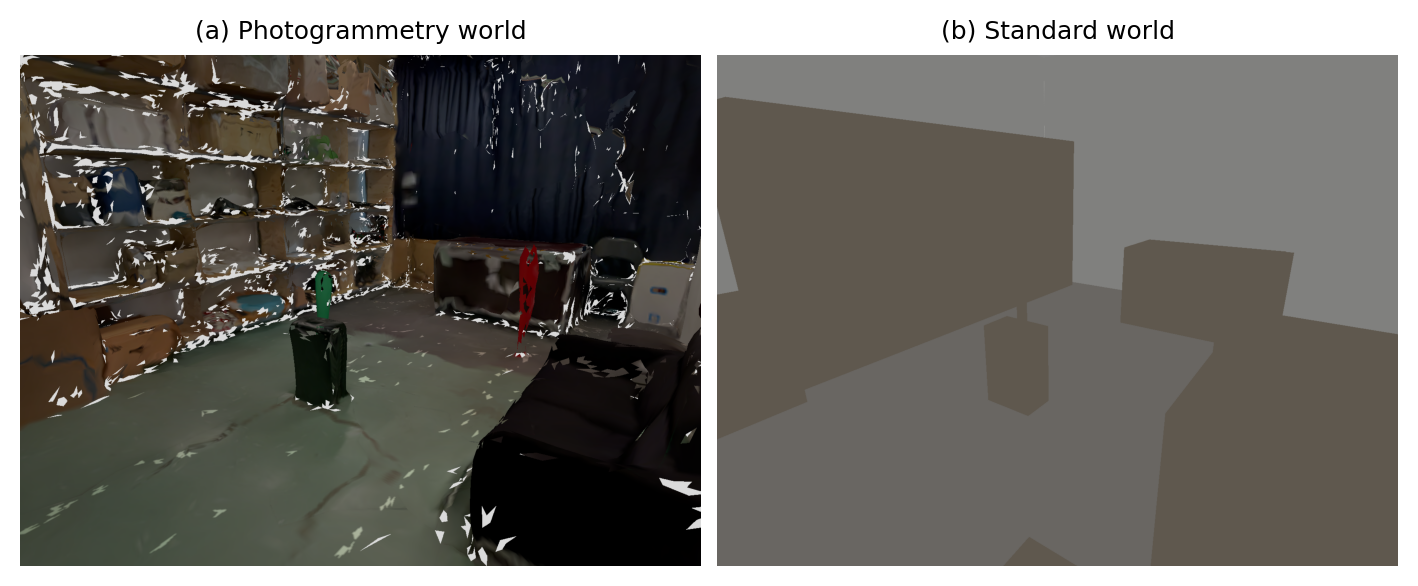
\includegraphics[width=\columnwidth]{figures/worlds}}%
{\fbox{\parbox[c][3cm][c]{0.9\columnwidth}{\centering\todo{figures/worlds.png: photogrammetry
world (left) and standard world (right), same viewpoint}}}}
\caption{The same view of the photogrammetry world (left) and the standard world (right). The
white flecks are texture artefacts from mesh decimation; they affect colour only, and the policy
observes depth.}
\label{fig:worlds}
\end{figure}

\subsection{Pepper in Simulation}
Pepper was simulated in Ignition Gazebo (Fortress) with ROS~2 Humble, using the DART physics engine
with Bullet collision detection and a 5\,ms step, and an open-source Pepper description that was
ported to ROS~2 Humble for this project. The policy uses only ROS 2 topics that also exist on the
real robot: the depth image from the head camera, the odometry of the base, and velocity commands to
the base. This means the same code drives both the simulated and the physical robot. The head was
fixed at a pitch of 0.45\,rad (looking down) in both simulation and reality. At Pepper's default
upward head angle, low obstacles such as the bag and the boxes leave the depth image when they are
still about 3\,m away.

Collisions are detected with contact sensors on eight links (base, torso, upper arms, forearms
and hands), and a tilt of more than $20^\circ$ is also treated as a collision (normal driving
never tilts Pepper by more than about $6^\circ$, so a larger tilt means the robot is falling
over). On the real robot,
the three base bumpers provide the same collision signal.

The simulated base was then calibrated against the real robot. The same set of velocity commands
(straight, reverse, spins and arcs) was sent to both, and their responses were compared. The real
robot reached its commanded speeds to within about 5\%, but responded with a median delay of 0.85\,s
through the full communication chain, while the simulated base responded almost instantly. The
simulator was therefore given a four-step (0.8\,s) command delay and acceleration limits fitted
to the real measurements.

\subsection{The Navigation Task}
The task is point-to-point navigation. Pepper starts at a pose in the room and must reach the red
goal pole, at $(3.75, 1.10)$\,m, without colliding. It is modelled as an MDP as follows.

\textbf{Observation.} At each step the policy receives:
\begin{itemize}
\item a $64\times48$ depth image, limited to 0.4--8.0\,m (the range of the simulated camera; the
real camera's readings were cut to the same range, and anything outside it, including missing
readings, is treated as far away);
\item the goal relative to the robot, as $(d, \sin\theta, \cos\theta)$, where $d$ is the distance
and $\theta$ the bearing;
\item the last six actions. Because commands take effect about 0.8\,s after they are sent, this
history tells the policy what it has already asked the robot to do.
\end{itemize}

\textbf{Action.} A continuous linear velocity $v\in[-0.10, 0.30]$\,m/s and angular velocity
$\omega\in[-0.90, 0.90]$\,rad/s, sent at 5\,Hz.

\textbf{Reward.} Each step's reward is
\begin{equation}
r_t = -0.05 + 20\,(d_{t-1}-d_t) - 0.02\,|\omega_t|,
\label{eq:reward}
\end{equation}
which consists of a small time penalty, a reward for every metre of progress towards the goal,
and a small penalty for turning. In addition, $+100$ is given for reaching the goal and $-100$ for
a collision.

\textbf{Episode end.} An episode ends when Pepper's base centre is within 0.6\,m of the goal
(success), when it collides or tips over, or after 120\,s.

\textbf{Starts and routes.} During training, each episode starts at a random collision-free position
with a random heading, so that the policy cannot memorise the validation starts. For evaluation, a
fixed set of 20 validation routes was generated (Fig.~\ref{fig:layout}). The shortest feasible path
length $\ell^*$ of each route was planned on the tape-measured map with obstacles enlarged by
0.32\,m to allow for Pepper's body. The same 20 routes are used for both branches, in simulation
and on the real robot. They were also used to choose which seed to deploy, so they are validation
routes rather than an untouched test set. Before the final training runs, short development runs
on them led to corrections of the simulation: the scanned floor was levelled, contact sensors were
added, the camera was tilted down to see low obstacles, and the goal tolerance and tip-over rule
were set. The action history and the latency, depth-noise and frame-rate randomisation were
added or set from measurements of the real robot rather than from route results. The reward,
network and SAC hyperparameters were set before the final training runs and not changed after.
The evaluations every 25{,}000 steps were used only for monitoring; the deployed policies are the
final ones at 300{,}000 steps.

\begin{figure}[t]
\centering
\IfFileExists{figures/layout.pdf}{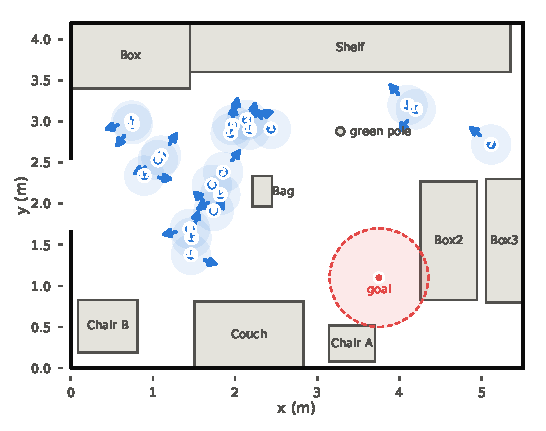
\includegraphics[width=\columnwidth]{figures/layout}}%
{\fbox{\parbox[c][4cm][c]{0.9\columnwidth}{\centering\todo{figures/layout.pdf: top-down room
plan with the 20 route starts and the goal zone}}}}
\caption{Top-down plan of the room with the 20 validation route starts (blue, arrows show the starting
heading) and the 0.6\,m goal zone around the red pole.}
\label{fig:layout}
\end{figure}

\subsection{Domain Randomisation}
Both branches were trained with the same randomisation (Table~\ref{tab:randomisation}). Each
parameter is sampled at the start of every episode and held fixed for that episode, following
Peng et al.\ \cite{peng2018dynamics}. Where possible, the ranges were set from measurements of the
real robot rather than chosen by hand. The command delay is varied around the measured 0.8\,s. The
depth noise matches the 5.5\,mm median frame-to-frame noise measured on the real camera. The
dropout patches imitate a full-height band with no depth readings that a window produced in the
real camera's image. The depth frame rate is varied because the real camera delivered only
1.9--3 frames per second over Wi-Fi during calibration, well below the 5\,Hz control rate. When
no new frame arrives, the policy receives the previous one again.

\begin{table}[t]
\caption{Randomisation applied during training, identical for both branches}
\label{tab:randomisation}
\centering
\footnotesize
\begin{tabular}{@{}llr@{}}
\toprule
Group & Parameter & Range \\
\midrule
\multirow{5}{*}{Command} & Linear / angular velocity scale & $\times$0.8--1.2 \\
 & Linear velocity noise (std) & 0.02\,m/s \\
 & Angular velocity noise (std) & 0.05\,rad/s \\
 & Command delay (around 4 steps) & $\pm$2 steps \\
 & Wheel slip probability & 0--0.05 \\
\midrule
\multirow{3}{*}{Depth} & Per-pixel noise (std) & 0.01\,m \\
 & Pixel and patch dropout & 0--15\% \\
 & Frame rate (log-uniform) & 1.5--15\,Hz \\
\midrule
Surface & Floor friction coefficient $\mu$ & 0.6--1.2 \\
\bottomrule
\end{tabular}
\end{table}

\subsection{Training with Soft Actor-Critic}
The policies were trained with the SAC implementation in Stable-Baselines3
\cite{haarnoja2018sac}, \cite{raffin2021sb3}. A small convolutional network, the
NatureCNN encoder from DQN \cite{mnih2015dqn}, encodes the depth image into 128 features, which are joined with the goal vector and action history and passed to
two fully connected layers of 256 units. The hyperparameters were the same for every run:
\begin{itemize}
\item learning rate $3\times10^{-4}$, discount $\gamma=0.99$, target update $\tau=0.005$;
\item replay buffer of 100{,}000 transitions, batch size 256, 2{,}000 warm-up steps;
\item one gradient step per environment step, and automatic entropy tuning;
\item 300{,}000 environment steps per run.
\end{itemize}

Three runs (seeds 0, 1 and 2) were trained per branch, six in total. One run takes 20--33 hours
of wall-clock time, so the runs were executed in parallel on the Wits mathematical sciences
cluster inside an Apptainer container. Training saved checkpoints every 25{,}000 steps and
resumed automatically when the simulator stalled. Every 25{,}000 steps, each run was evaluated
once on the 20 routes.

After training, each final policy was evaluated in its own world over five independent sessions
of the 20 routes. Several sessions are needed because the simulator runs in real time rather
than in fixed steps, so repeated runs of the same policy do not give identical results. Before
any real-robot run, a rule was fixed for choosing which policy from each branch to deploy: the
seed with the highest simulated SR, with ties broken by SPL. This selected standard seed~1 and
photogrammetry seed~0.

\subsection{Deployment on the Real Pepper}
The policies were deployed zero-shot, with no fine-tuning on the real robot. Pepper's software
(NAOqi 2.5) supports only Python 2.7 for its Python SDK, so a small Python~2 program on the laptop
talks to the robot over the network, and a ROS~2 bridge node republishes its data under the same
topic names as the simulator. The policy therefore runs unchanged. The depth image ($160\times120$
requested at 5\,Hz), odometry, bumper states and velocity commands all pass through this link. As a
safety measure, the robot stops if no command arrives for 1.5\,s, and the emergency stop button was
always within reach. For safety, NAOqi's built-in collision protection, which slows or stops the
base near obstacles, was kept on for all real trials.

The 20 routes were taped onto the floor of the real room. For each route, the operator placed Pepper
on the taped start, and its odometry was reset to that known pose. The policy then ran until
success, collision or 120\,s. Contacts that the base bumpers cannot detect, such as an arm brushing
furniture, were noted by the operator. The evaluation took place over two days (routes r000--r010
and r011--r019), and the order of the two policies was swapped on the second day.

\subsection{Evaluation Metrics}
Four metrics are used. Over the $N=20$ routes, the \emph{success rate} is
$\mathrm{SR}=\frac{1}{N}\sum_i S_i$, where $S_i=1$ if route $i$ ended within 0.6\,m of the goal with
no collision before the time limit, and 0 otherwise. On the real robot, no external tracking was
available, so whether a route succeeded and the distance travelled both come from odometry, reset at
the taped start of each route. We call this odometry-estimated success. Real-robot SR and SPL are
therefore odometry-estimated, and the sim-to-real gap compares them with simulated values computed
from the true pose.

The \emph{success weighted by path length} \cite{anderson2018evaluation} also rewards efficient
paths:
\begin{equation}
\mathrm{SPL}=\frac{1}{N}\sum_{i=1}^{N} S_i\,\frac{\ell^*_i}{\max(\ell_i,\ell^*_i)},
\label{eq:spl}
\end{equation}
where $\ell_i$ is the distance actually travelled. The \emph{collision rate} CR is the number of
collisions per metre travelled. The \emph{sim-to-real gap} for a metric $M$ is
\begin{equation}
\Delta M = M_{\text{sim}} - M_{\text{real}},
\label{eq:gap}
\end{equation}
computed separately for each branch. A smaller $\Delta$ means the simulator predicted real
performance better.

The main comparison is between branches: photogrammetry is considered better if
$\Delta_{\text{photo}}$ is smaller than $\Delta_{\text{std}}$. This is tested per route with the
Wilcoxon signed-rank test ($\alpha=0.05$) on the paired differences
$\Delta_{\text{photo},i}-\Delta_{\text{std},i}$, where a route's gap is its mean simulated outcome
over the five sessions minus its real outcome. Real-robot performance of the two policies is also
compared directly. Both tests pair each route with itself, because both branches use the same
20 routes. The same paired test checks whether each branch's own gap is larger than zero. 95\%
confidence intervals for the real-robot SR use the Wilson score interval.
